%!TEX program = pdflatex
\documentclass[UTF8]{beamer}
\usepackage{ctex}
\usepackage{hyperref}
\usepackage{CJKutf8}
\usepackage{times}
\usepackage[english]{babel}
\usepackage{color}
\usepackage{graphicx}
\usepackage{url}
\usepackage{bm}
\usepackage{tikz}

\usetheme{CambridgeUS}
\usefonttheme{serif}
\newcommand{\lcp}{\operatorname{lcp}}
\newcommand{\suf}{\operatorname{suf}}

\begin{document}
\begin{CJK}{UTF8}{song}
\title[字符串]{字符串}

\author{Flying2018}
\date{\today}

\begin{frame}
	\titlepage
\end{frame}
%\begin{frame}
%  \frametitle{目录}
%  \tableofcontents[hideallsubsections]
%\end{frame}
\section{前置知识}
\begin{frame}
	\par
	\textbf{以下默认大家熟练掌握了的算法:}
	\begin{itemize}
		\item Hash
		\item Trie树
		\item KMP
		\item 平衡树(除 Splay 外)
		\item 倍增,计数排序,单调栈
	\end{itemize}
\end{frame}
\begin{frame}
	\frametitle{一些比较靠谱的记号}
	\begin{itemize}
		\item 默认字符串下标从1开始。
		\item $\Sigma$ 表示字符集大小。
		\item $|s|$ 表示字符串 $s$ 的长度。
		\item $s[i:j]$ 表示 $s$ 串的由区间 $[i,j]$ 中字符构成的子串,即 $s_is_{i+1}\cdots s_{j}$。
		\item 特别的,对于前缀 $s[1:i]$ 我们简写作 $s[:i]$,对于后缀 $s[i:|s|]$ 简写作 $s[i:]$。
		\item 设两个字符串 $s,t$,$s+t$ 表示 $s$ 和 $t$ 按顺序拼接的结果,即 $s_1s_2\cdots s_{|s|}t_1t_2\cdots t_{|t|}$。
		\item 设两个字符串 $s,t$,$s<t$ 表示对 $s$ 和 $t$ 的字典序比较时 $s$ 字典序较小。$s=t$ 表示 $s$ 和 $t$ 本质相同。
		\item $\texttt{(sth)}$ 表示 $\texttt{sth}$ 对应的字符。$s+\texttt{(c)}$ 表示在 $s$ 末尾加上字符 $\texttt{c}$ 。
	\end{itemize}
\end{frame}

\section{后缀数组}
\begin{frame}
	\frametitle{后缀数组}
	\par
	\begin{block}{后缀排序}
		给定一个长度为 $n$ 的字符串 $s$。\\
		求出一个数组 $sa_i$,满足 $\forall 1\leq x<y<n,s[sa_x:]<s[sa_y:]$。\\
	\end{block}
	\pause
	\par 即:把字符串 $s$ 的所有非空后缀按字典序从小到大排序。
\end{frame}
\subsection{二分 Hash 后缀数组}
\begin{frame}
	\frametitle{一个 simple 的想法}
	\pause
	\par
	一个 simple 的 $O(n\log^2 n)$ 做法:\\
	使用 Hash,暴力二分处理两两串的 ${\lcp}$。直接套用快速排序。
	\pause
	\par
	单次比较 $O(\log n)$,需要比较 $O(n\log n)$ 次。\\
	总复杂度 $O(n\log^2 n)$。\\
	虽然没什么用,但这个算法可以给我们一些启发。
\end{frame}
\subsection{倍增后缀数组}
\begin{frame}
	\frametitle{优化?}
	考虑我们是如何暴力比较两个字符串的字典序大小的?
	\pause
	\par
	对于后缀 $s[i:],s[j:]$,假如我们已经知道 $s[i:i+k-1]=s[j:j+k-1]$。那么我们是不是只需要判断 $s[i+k:],s[j+k:]$ 的字典序就好了?
\end{frame}
\begin{frame}
	\frametitle{倍增后缀数组}
	我们现在排的字符串是 $s[i:i+k-1],i\in[1,n]$,如果 $i+k>n$ 就视为 $s[i:]$。
	记数组 $rk_i$ 表示当前的 $s[i:]$ 的排名。
	\pause
	\par
	很明显,$rk_i<rk_j\Rightarrow s[i:]<s[j:]$。\\
	\pause
	\par
	而对于 $rk_i=rk_j$,如果 $rk_{i+k}\neq rk_{j+k}$,那么也可以推出 $s[i:]$ 与 $s[j:]$ 的大小关系。
\end{frame}
\begin{frame}
	\frametitle{具体实现}
	\pause
	\par
	\begin{figure}[h]
		\centering
		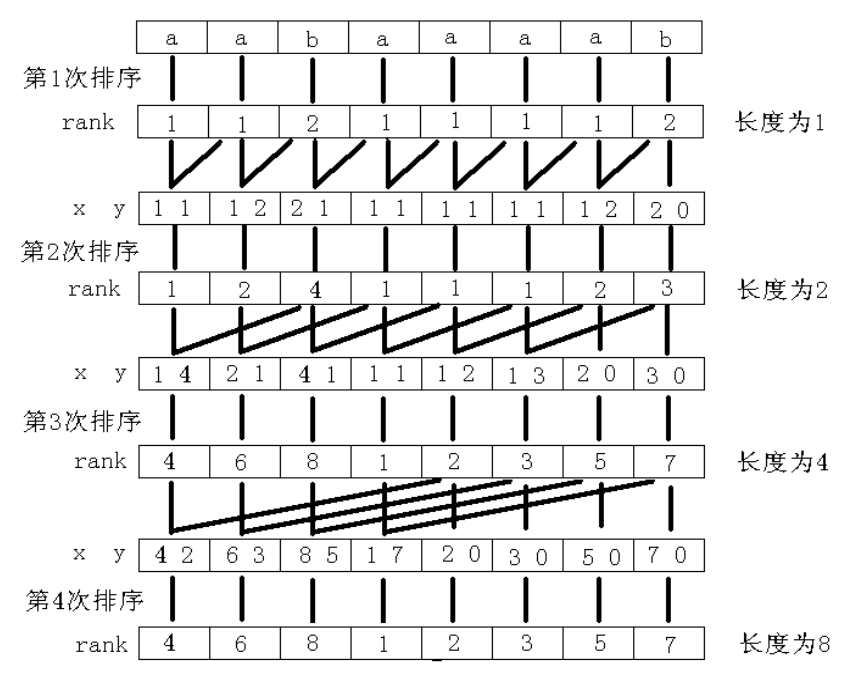
\includegraphics[width=0.7\linewidth]{figures/sa.png}
	\end{figure}
%	\pause
%	\par
%	采用基数排序。\\
%	我们把 $rk_i$ 当做第一关键字加入桶中,把 $rk_{i+k}$ 作为排序依据在每个桶中排序。
%	\pause
%	\par
%	注意这里用到一个小 trick。我们可以用上一轮排好的 sa 数组,先排出只以 $rk_{i+k}$ 作为排序依据时的结果。\\
%	然后我们从前往后按顺序将这个数组中的元素插入对应的桶 $rk_i$ 中。
%	\pause
%	\par
%	排序完成之后用新的 sa 求出新的排名,注意这里需要去重。判重方式很简单,即对于桶中相邻项 $i,j$,判断是否有 $rk_i=rk_j$ 且 $rk_{i+k}=rk_{j+k}$。\\
%	同时 $k\leftarrow 2\times k$。\\
%	\pause
%	\par
%	重复上述步骤直到不存在重复元素。单次排序 $O(n)$,最坏处理 $O(\log n)$ 次,总复杂度 $O(n\log n)$。
%	\pause
%	\par
%	实际代码其实非常短。
\end{frame}
\subsection{height 数组}
\begin{frame}
	\frametitle{height 数组}
	\pause
	\par
	单独求出 $sa_i$ 好像没有什么太大用处,至少没有出题人会让你输出 $sa_i$。
	\par
	所以我们需要一些扩展的东西让后缀数组变得有用一些。
	\pause
	\par
	为了方便表示,我们用 $\suf_i$ 表示后缀排序后的第 $i$ 个后缀,即 $s[sa_i:]$。
	\begin{block}{height 数组}
	$height_i$ 表示 $\lcp(\suf_{i-1},\suf_{i})$。\\
	即 $sa$ 数组中相邻两个后缀的 $\lcp$。
	\end{block}
\end{frame}
\begin{frame}
	\frametitle{特殊性质}
	\begin{block}{性质}
		$\forall i,j\in[1,n],j-i>1$\\
		$\lcp(\suf_i,\suf_j)=\min\{\lcp(\suf_{i},\suf_{k}),\lcp(\suf_k,\suf_j)\},k\in(i,j)$
	\end{block}
	\pause
	\par
	证明比较显然,具体可以考虑第 $\lcp(\suf_i,\suf_j)+1$ 个字符的情况。
	\pause
	\begin{block}{推论1}
		$\forall i,j\in[1,n],j-i>1$\\
		$\lcp(\suf_i,\suf_j)=\min_{k\in(i,j]}\{height_k\}$
	\end{block}
	\begin{block}{推论2}
		$\forall i<j\leq n,height_{i+1}\geq\lcp(\suf_i,\suf_j)$
	\end{block}
\end{frame}
\begin{frame}
	\frametitle{如何求 height 数组}
	\pause
	\begin{block}{定义 h 数组}
		$h_i=height[rk_i]$
	\end{block}
	\pause
	\begin{block}{一个性质}
		$\forall 1<i\leq n,h_{i}\geq h_{i-1}-1$
	\end{block}
	\pause
	\begin{block}{简要证明}
		设 $k=sa[rk[i-1]-1]$,即排在 $s[i-1:]$ 前一名的后缀,则 $h_{i-1}=\lcp(s[k:],s[i-1:])$。\\
		如果 $h_{i-1}\leq 1$,结论显然成立。\\
		否则去掉第一个字符,有 $\lcp(s[k+1:],s[i:])=h_{i-1}-1$。\\
		由于 $\lcp(s[k:],s[i-1:])>1$,有 $rk_k<rk_{i-1}\Rightarrow rk_{k+1}<rk_{i}$。\\
		由上一页推论2,有 $\lcp(s[i:],s[k+1:])\leq h_i$。\\
		于是我们推出 $h_i\geq h_{i-1}-1$。
	\end{block}
\end{frame}
\begin{frame}
	\frametitle{如何求 height 数组}
	然后我们就知道了:按照 $rk$ 的顺序求出 height 数组,暴力求 $\lcp$ 的时间复杂度是 $O(n)$。
	代码同样非常简短。
\end{frame}
\subsection{扩展}
\begin{frame}
	\frametitle{一些扩展}
	\pause
	\begin{block}{处理多串问题}
		后缀排序是可以直接将多个串按上述方式处理的。但可能需要特殊处理全等的情况。\\
		比较常见的方法是在每个字符串最后添加一个字符 $?$(字典序要小于所有字符)然后将所有串拼接起来。
	\end{block}
\end{frame}
\begin{frame}
	\frametitle{一些扩展}
	\begin{block}{本质不同子串}
		不妨钦定所有重复出现的子串都“属于”字典序最小的那个后缀。\\
		可以发现答案就是 $\frac{n(n+1)} 2-\sum{height_i}$。
	\end{block}
	\pause
	\begin{block}{height rmq}
		由于 height 数组的特殊性质,常常会遇到 height rmq 的问题。\\
		假如我们把平面上 $(i,[1,height_i])$ 部分的点染黑。可以发现大部分问题都可以转换为子矩形问题。\\
		可以用单调栈/二分处理。
	\end{block}
\end{frame}
\subsection{例题}
\begin{frame}
	\frametitle{一些例题}
	以下例题均可以用 SAM 秒杀。\\
	最好思考一下用 SA 怎么做。
\end{frame}
\begin{frame}
	\frametitle{Fake News}
	\begin{block}{题意}
		给定一个字符串 $s$。求 $s[i:j]=s[l:r]$ 数量。
	\end{block}
	\pause
	\par
	可以看成 $\sum_{i<j}\lcp(s[i:],s[j:])$。\\
	由 height 性质可以变成 $\sum_{i<j}\sum_{k\in(i,j]}height_k$。\\
	转换为子矩形问题,单调栈处理。\\
	时间复杂度 $O(n\log n)$。
\end{frame}
\begin{frame}
	\frametitle{弦论}
	\begin{block}{题意}
		给你一个字符串,问:\\
		1. 本质不同子串中字典序第 $k$ 小的子串是什么。\\
		2. 所有 $\frac {n(n+1)}2$ 个子串中第 $k$ 小的子串是什么。
	\end{block}
	\pause
	\par
	询问 1 就是 SA 的基操。重点在于处理询问 2。
	\pause
	\par
	如果按照询问 1 的思路,我们需要求出每个本质不同子串的出现次数。转换为上一题的套路。\\
	用单调栈解决。总复杂度 $O(n\log n)$。
\end{frame}
\begin{frame}
	\frametitle{品酒大会}
	\begin{block}{题意}
		给你一个长度为 $n$ 的字符串 $s$,对于所有 $l\in[0,n-1]$ 问:\\
		1. $\sum_{i<j}[\lcp(s[i:],s[j:])\leq l]$\\
		2. $\max_{i<j}[\lcp(s[i:],s[j:])\leq l]v_iv_j$\\
		$n\leq 3\times 10^5,|v_i|\leq 10^9$。
	\end{block}
	$\leq l$ 限制可以先看做 $=l$ 限制,最后后缀处理一下即可。\\
	对于询问1,显然就是之前的套路,只不过每次改为更新 $height_i$ 位置的答案而已。\\
	\pause
	对于询问二,可以发现乘积最大值一定是由最大的两个值或是最小的两个值相乘得到。\\
	同样可以转换成数矩形问题,单调栈维护。\\
	总复杂度 $O(n\log n)$。
\end{frame}
\subsection{}
\begin{frame}
	可以发现以上问题的复杂度瓶颈似乎都在于求后缀数组,求出后缀数组之后似乎都可以 $O(n)$ 求出答案。\\
	然而倍增后缀数组太拖后腿了,导致复杂度直接变成 $O(n\log n)$。\\
	那么有没有 $O(n)$ 求后缀数组的方法呢?\\
	\pause
	\par
	肯定是有的。现在比较常用的算法是 SA-IS,复杂度严格 $O(n)$,可以优化一半左右的时间。\\
\end{frame}
\begin{frame}
	\begin{figure}[h]
		\centering
		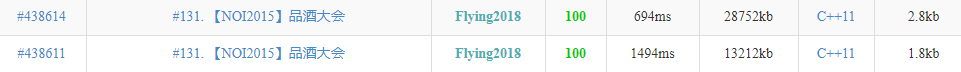
\includegraphics[width=1.0\linewidth]{figures/compare.png}
	\end{figure}
	优化还是挺明显的。\\
	\pause
	\par
	然而优化时间复杂度对大部分题目帮助不大。很少会遇到出题人故意把字符串开到 $10^7$ 卡掉 SA。
\end{frame}
\begin{frame}
	SA 有一个更为关键的缺陷:它是一个离线算法。
	\pause
	\par
	这导致 SA 的通用性大大降低。\\
	所以我们希望有一个动态维护后缀数组的算法。
\end{frame}
\section{后缀平衡树}
\begin{frame}
	\frametitle{在线化的后缀数组}
	\pause
	\par
	用数组维护后缀之间的相对位置太 simple 了。\\
	考虑用一个平衡树去维护。
	\pause
	\par
	但是这样倍增就失效了,所以我们需要其他的方法来维护。
\end{frame}
\subsection{二分 Hash 后缀平衡树}
\begin{frame}
	\frametitle{一个 simple 的做法}
	首先我们还是考虑比较 simple 的 Hash。\\
	每次插入一个后缀我们直接用 Hash 二分比较字典序。
	\pause
	\par
	单次 $O(\log^2 n)$,总复杂度 $O(n\log^2 n)$。
\end{frame}
\subsection{$O(\log n)$ 后缀平衡树}
\begin{frame}
	\frametitle{优化}
	但是上面那个做法太 naive 了,完全没有用到后缀连续的性质。
	\pause
	\par
	假设我们是倒序(从后往前)插入。\\
	可以发现,当我们比较 $s[i:]$ 和 $s[j:]$ 时,$s[i+1:]$ 和 $s[j+1:]$ 已经被插入了。\\
	按照暴力比较的思路,假如 $s_i= s_j$,我们直接比较 $s[i+1:]$ 和 $s[j+1:]$ 即可。
\end{frame}
\begin{frame}
	\frametitle{具体实现}
	后缀平衡树每个点维护一个相对权值,即:$V_u\leftarrow (V_{lson}+V_{rson})/2$。\\
	这样就保证了 $V$ 满足中序递增。就可以 $O(1)$ 比较权值。
	\pause
	\par
	总复杂度 $O(n\log n)$。
	\pause
	\par
	由于要保证 $V$ 值域平衡,这里需要使用重量平衡树,即任何时刻树深都是 $O(\log n)$ 级别的。\\
	一般情况写替罪羊树会比较方便。\\
	当然,遇到可持久化的情况一般选择非旋treap。
\end{frame}
\subsection{扩展}
\begin{frame}
	\frametitle{一个扩展}
	上述的后缀平衡树算法也可以扩展到 trie 上。\\
	具体也很简单,就是每次找到要扩展的那个后缀,然后按上面的方式加入扩展后的后缀即可。
\end{frame}
\subsection{例题}
\begin{frame}
	\frametitle{Phorni}
	\begin{block}{题目大意}
	维护一个 $n$ 个元素的序列 $a_i$,每个元素是字符串 $s$ 的一个后缀。\\
	支持:在 $s$ 开头加一个字符,改变某个 $a_i$ 表示的后缀位置,求 $i\in [l,r]$ 字典序最小的 $a_i$ 编号(如有相同输出编号最小)。强制在线。
	\end{block}
	\pause
	\par
	用平衡树维护各后缀之间的相对位置,然后用一颗线段树处理 $n$ 个后缀的相对权值即可。
	总复杂度 $O(|s|\log |s|+n\log n)$。
\end{frame}
\begin{frame}
	\frametitle{ydc的字符串}
	\begin{block}{题目大意}
	定义 $s$ 通过 $[l,r]$ 与 $t$ 相等,当且仅当在 $s$ 串末尾添加一个 $[l,r]$ 区间内的字符后和 $t$ 全等。
	\pause
	\par
	给定 $n(n\leq 5)$ 个字符串,$q$ 次操作,支持:
	\begin{itemize}
	\item 在某个字符串后面加上一个字符。
	\item 问第 $x$ 个字符串有多少个子串通过 $[l,r]$ 与第 $k$ 次操作后的第 $y$ 个字符串x相等。
	\item 将第字符串 $x$ 改为第 $y$ 个字符串。
	\item 给定一个模式串 $s$,对于当前每个串询问有多少个子串能使得 $s$ 通过 $[l,r]$ 相等。
	\end{itemize}
	强制在线。
	$q\leq 2\times10^5,\sum|s|\leq 10^6$。
	\end{block}
\end{frame}
\begin{frame}
	\frametitle{ydc的字符串}
	\begin{block}{一个常见的套路}
	\pause
	\par
	对于“在 $[l,r]$ 内的出现次数”这类问题,一般都是可差分的,即转换为 $[1,r]$ 内出现次数减去 $[1,l-1]$ 的出现次数。
	\pause
	\par
	比如询问一个字符串 $s$ 在字符串 $t[l:r]$ 的出现次数,我们就可以转换为在 $t[:r]$ 的出现次数减去 $t[:l-1]$ 的出现次数。\\
	于是就可以用一个可持久化后缀平衡树来维护。
	\end{block}
	\pause
	\par
	而这道题,显然就是特意为后缀平衡树构造的。因为对于询问串 $s$,我们只需要用 $s+\texttt{(r+1)}$ 的排名减去 $s+\texttt{(l)}$ 的排名就是答案。
	\pause
	\par
	于是这道题就可以用一个 Hash 版本的可持久化后缀平衡树来做到 $O(q\log^2 |s|)$。
\end{frame}
\begin{frame}
	\frametitle{STRQUERY}
	\begin{block}{题目大意}
	维护一个字符串,开始时为空串。共 $n$ 次操作,支持:前端加/删字符,后端加/删字符,正中间 $(\lceil\frac{|s|} 2\rceil)$ 加/删字符,查询某个字符串 $t$ 在 $s$ 中的出现次数。\\
	$n\leq 1.5\times 10^5,\sum |t| \leq 1.5\times 10^6$。\\
	强制在线。
	\end{block}
\end{frame}
\begin{frame}
	\frametitle{STRQUERY}
	看着很麻烦,尤其是“中间加/删”。我们不妨先考虑前/后端加/删的情况。
	\pause
	\par
	按照套路,我们将队列从某一位置拆开,转化成两个栈。这样我们就可以通过后缀平衡树分别维护两个栈的信息。\\
	如果一个栈空了,就把另一边的一半扔进来。可以证明这样均摊是 $O(n\log n)$ 的。\\
	对于中间的,可以发现需要匹配的长度只有 $O(|t|)$,直接取出暴力 KMP 即可。\\
	复杂度 $O((n+|t|)\log n)$。
\end{frame}
\begin{frame}
	\frametitle{STRQUERY}
	那么中间加/删怎么处理?\\
	\pause
	\par
	考虑我们从中间划一刀,对左右部分分别使用上述的方式维护。那么中间加/删可以转化为 $O(1)$ 次左右加/删。\\
	最后中间部分再进行一次暴力 KMP。时间复杂度同样是 $O((n+|t|)\log n)$。
\end{frame}
\section{}
\begin{frame}
	\frametitle{The end}
	谢谢大家。
\end{frame}
\end{CJK}
\end{document}